\documentclass[12pt]{article}
\usepackage{fullpage,enumitem,amsmath,amssymb,graphicx}
\usepackage{graphicx} % This is a package for including graphics in your solution.
\usepackage{listings}
\usepackage[final]{pdfpages}

\begin{document}

\begin{center}
{\Large CS168 Spring Assignment 3}

\begin{tabular}{rl}
SUNet ID(s): 05794739 & \\
Name(s): & Luis A. Perez \\
Collaborators: &
\end{tabular}
\end{center}

By turning in this assignment, I agree by the Stanford honor code and declare
that all of this is my own work.

\section*{Part 1}

\begin{enumerate}[label=(\alph*)]
  \item
    Objective value of LS Solution: 226.66
    Objective value of zero solution: 73311.60
  \item
    The gradient of $f$ for $\mathbf{a}$ is given by:
    \begin{align*}
      \frac{d}{d\mathbf{a}} f(\mathbf{a}) &= \frac{d}{d\mathbf{a}}\left[ \sum_{i=1}^n f_i(\mathbf{a})\right] \tag{Definition of $f$} \\
      &=  \sum_{i=1}^n \frac{d}{d\mathbf{a}} f_i(\mathbf{a}) \tag{Properties of derivatives} \\
      &= \sum_{i=1}^n \frac{d}{d\mathbf{a}} (\mathbf{a}^T\mathbf{x}^{(i)} - y^{(i)})^2 \\
      &= 2 \sum_{i=1}^n  \mathbf{x}^{(i)}(\mathbf{a}^T\mathbf{x}^{(i)} - y^{(i)}) \\
    \end{align*}
    \[
      \frac{d}{d\mathbf{a}} f(\mathbf{a}) = 2\mathbf{X}^T (\mathbf{X}\mathbf{a} - \mathbf{y})
    \]
    where $\mathbf{X} \in \mathbb{R}^{n \times d}$ has each row as $\mathbb{x}^{(i)}$ and $\mathbb{1} \in \mathbb{R}^d$ is a vector of all $1$s.

  The code used for our solution:
\begin{verbatim}
def gradient(X, y, ahat):
    """Computes the gradient of the cost_function above."""
    return 2 * np.dot(X.T, np.dot(X, ahat) - y)

def initialize_params(d:int):
    """Returns initial parameters to use during gradient descent.
    
    Args:
        d: The dimension of the feature space.
    """
    return np.zeros((d, 1))
    
def gradient_descent(X, y, step_size: float, n_iters: int = 20):
    """Runs gradient descent on data.
    
    Args:
        X, y: The data and labels.
        step_size: Size of step to take in direction of gradients.
        n_iters: Number of iterations of gradient descent.
        
    Returns the parameters after n_iters and a list of n_iters + 1
        elements where costs[i] corresponds to the objective value
        after i iterations.
    """
    _, d = X.shape
    a_hat = initialize_params(d)
    costs = [cost_funtion(X, y, a_hat)]
    for _ in range(n_iters):
        a_hat = (a_hat - step_size * gradient(X, y, a_hat))
        costs.append(cost_funtion(X, y, a_hat))
        
    return costs, a_hat

def plot_training(step_sizes, optimizer, title):
    plt.title("Objective Value after some number of iterations")
    plt.ylabel("Objective Value")
    plt.xlabel("Iteration")
    for step_size in step_sizes:
        costs, _ = optimizer(Globals.X, Globals.y, step_size)
        print("[step_size={}] Objective value: {:.4f}".format(step_size, costs[-1]))
        plt.plot(range(len(costs)), costs, label="step_size=%s" % step_size)

    plt.legend()
    plt.savefig("figures/%s.png" % title, format='png')
    plt.close()

def problem1b():
    plot_training([0.00005, 0.0005, 0.0007], optimizer=gradient_descent, title="gradient_descent_all")
    plot_training([0.00005, 0.0005], optimizer=gradient_descent, title="gradient_descent_converge")

problem1b()
\end{verbatim}

    The above code results in Figure \ref{fig:gradient_descent_all} for the three specified step sizes. For clarity, we also plot Figure \ref{fig:gradient_descent_convergent}, which only focuses on the two step sizes that converge.
    \begin{figure}[!ht]
      \centering
      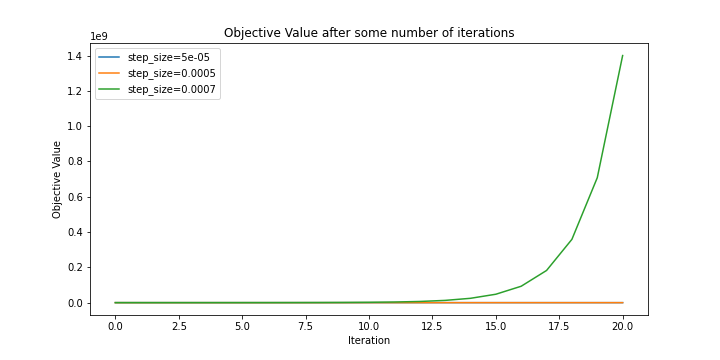
\includegraphics[scale=0.5]{figures/gradient_descent_all.png}
      \caption{Objective value using gradient descent for multiple step sizes.}
      \label{fig:gradient_descent_all}
    \end{figure}
    \begin{figure}[!ht]
      \centering
      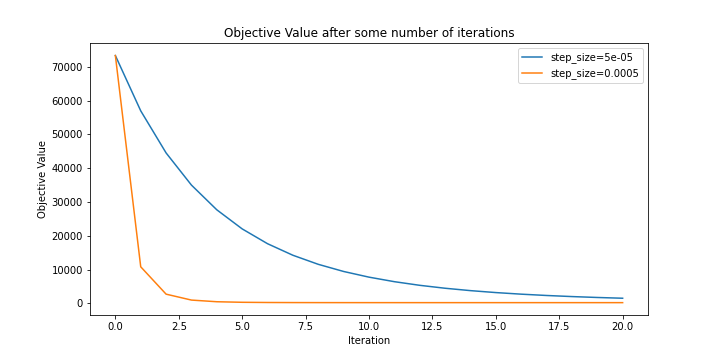
\includegraphics[scale=0.5]{figures/gradient_descent_converge.png}
      \caption{Objective value using gradient descent for convergent step sizes.}
      \label{fig:gradient_descent_convergent}
    \end{figure}

    The optimal step size if $0.0005$, which achieves objective value of 226.6593 (matching the analytical solution).


    From the above, we can see that the step size is a critical parameter to select. A step size that's too large (such as 0.0007) leads to the algorithm diverging, likely due to the fact that the steps consistently overshoot any local minimum. However, too small a step size such as 0.00005 leads to optimization that's significantly slower (as we can see in Figure \ref{fig:gradient_descent_convergent}), and which actually ends with a higher objective value. The optimal step size is therefore a sweet spot that can't be too large or too small.

  \item
    The code used builds on top of that for part (b). We present the modifications below:
    \begin{verbatim}
def norm_error(X, y, a):
    """Computes normalized error."""
    return np.linalg.norm(np.dot(X, a) - y) / np.linalg.norm(y)

def sgd(X, y, step_size: float, n_iters: int = 1000, include_cost:bool=True,
        include_detail=False, X_test=None, y_test=None, initializer=initialize_params):
    """Runs stochastic gradient descent on data.
    
    Args:
        X, y: The data and labels.
        step_size: Size of step to take in direction of gradients.
        n_iters: Number of iterations of gradient descent.
        
    Returns the parameters after n_iters and a list of n_iters + 1
        elements where costs[i] corresponds to the objective value
        after i iterations.
    """
    n, d = X.shape
    a_hat = initializer(d)
    costs = [cost_funtion(X, y, a_hat)] if include_cost else None
    normed_train_error = [norm_error(X, y, a_hat)] if include_detail else None
    normed_test_error = [norm_error(X_test, y_test, a_hat)] if include_detail else None
    l2_norm = [np.linalg.norm(a_hat)] if include_detail else None
    indexes = np.random.randint(0, high=n, size=n_iters)
    for i, idx in enumerate(indexes):
        a_hat = (a_hat - step_size * gradient(np.take(X, [idx], axis=0), np.take(y, [idx], axis=0), a_hat))
        if include_cost:
            costs.append(cost_funtion(X, y, a_hat))
        if include_detail and i % 100 == 0:
            normed_train_error.append(norm_error(X, y, a_hat))
            normed_test_error.append(norm_error(X_test, y_test, a_hat))
            l2_norm.append(np.linalg.norm(a_hat))
            
    if not include_detail:
        return costs, a_hat
    return costs, a_hat, normed_train_error, normed_test_error, l2_norm

def problem1c():
    plot_training([0.0005,0.005,0.01], optimizer=sgd, title="sgd_all")
    plot_training([0.0005,0.005], optimizer=sgd, title="sgd_converge")

problem1c()
    \end{verbatim}
    
    The above code results in Figure \ref{fig:sgd_all} for the three specified step sizes. For clarity, we also plot Figure \ref{fig:sgd_convergent}, which only focuses on the two step sizes that converge.
    \begin{figure}[!ht]
      \centering
      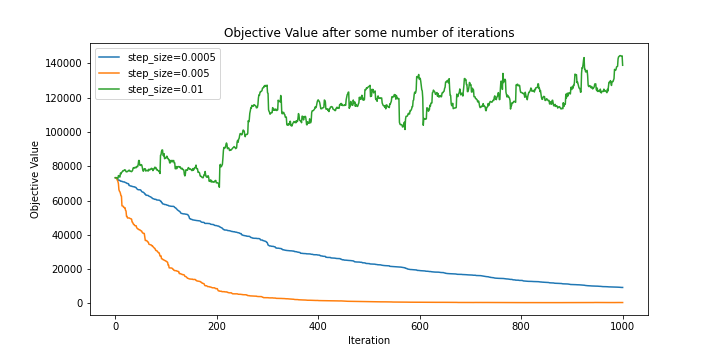
\includegraphics[scale=0.5]{figures/sgd_all.png}
      \caption{Objective value using gradient descent for multiple step sizes.}
      \label{fig:sgd_all}
    \end{figure}
    \begin{figure}[!ht]
      \centering
      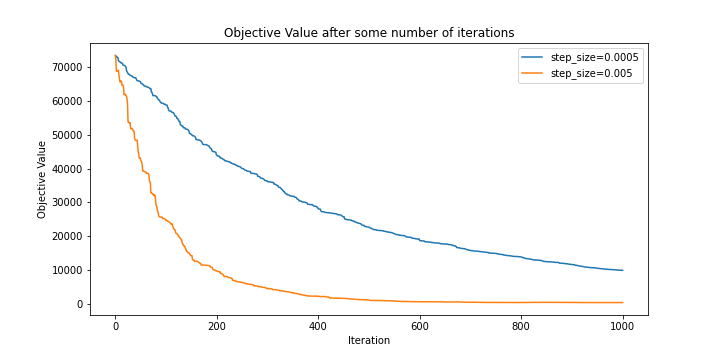
\includegraphics[scale=0.5]{figures/sgd_converge.png}
      \caption{Objective value using gradient descent for convergent step sizes.}
      \label{fig:sgd_convergent}
    \end{figure}

    The optimal step size if $0.005$, which achieves objective value of 423.2765 (worse than the analytical solution, but somewhat better).


    From the above, we can see that the step size is a critical parameter to select. A step size that's too large (such as 0.01) leads to the algorithm diverging, likely due to the fact that the steps consistently overshoot any local minimum since SGD is quite noisy. However, too small a step size such as 0.0005 leads to optimization that's significantly slower (as we can see in Figure \ref{fig:gradient_descent_convergent}), and which actually ends with a high objective value. The optimal step size is therefore a sweet spot that can't be too large or too small.

\end{enumerate}

\newpage
\section*{Part 2}
\begin{enumerate}[label=(\alph*)]
  \item

    The code used is presented below.
    \begin{verbatim}
def generate_data_2():
    train_n = 100
    test_n = 1000
    d = 100
    X_train = np.random.normal(0,1, size=(train_n,d))
    a_true = np.random.normal(0,1, size=(d,1))
    y_train = X_train.dot(a_true) + np.random.normal(0,0.5,size=(train_n,1))
    X_test = np.random.normal(0,1, size=(test_n,d))
    y_test = X_test.dot(a_true) + np.random.normal(0,0.5,size=(test_n,1))
    
    return X_train, y_train, X_test, y_test, a_true

def linear_solver(X, y):
    """Analytical solution for linear regression of square matrix."""
    return np.dot(np.linalg.inv(X), y)

def train_test_error(X_train, y_train, X_test, y_test, a_true, solver):
    """Returns train/test error for simple linear regression."""
    # Complex formulay covers the special case of the simple formula.
    a_hat = solver(X_train, y_train)
    train_error = norm_error(X_train, y_train, a_hat)
    train_true_error = norm_error(X_train, y_train, a_true)
    test_error = norm_error(X_test, y_test, a_hat)
    test_true_error = norm_error(X_test, y_test, a_true)
    return train_error, test_error, train_true_error, test_true_error

def avg_train_test_error(n_trials, solver):
    """Using provided solver, run n_trails and report average train/test errors (normalized)."""
    errors = [train_test_error(*generate_data_2(), solver=solver)
              for _ in range(n_trials)]
    train_errors, test_errors, train_true_errors, test_true_errors = zip(*errors)
    avg_train_error, avg_test_error = np.mean(train_errors), np.mean(test_errors)
    avg_train_true_error, avg_test_true_error = np.mean(train_true_errors), np.mean(test_true_errors)
    return avg_train_error, avg_test_error, avg_train_true_error, avg_test_true_error

def problem2a():
    train, test, train_true, test_true = avg_train_test_error(n_trials=10, solver=linear_solver)
    print("Average normalized train error: {:.4f} compared to true train error: {:.4f}".format(train, train_true))
    print("Average normalized test error: {:.4f} compared to true test error: {:.4f}".format(test, test_true))

problem2a()
    \end{verbatim}
    Average normalized train error: 0.0000 compared to true train error: 0.0517
    
    Average normalized test error: 1.2890 compared to true test error: 0.0495

  \item
    The code used is presented below (used in conjunction with previous code).
    \begin{verbatim}
def l2_regularized_solver(X, y, reg_coeff):
    n, _ = X.shape
    invertible = np.dot(X.T, X) + reg_coeff * np.identity(n)
    return np.dot(np.dot(np.linalg.inv(invertible), X.T), y)

def problem2b():
    errors = []
    coeffs = [0.0005,0.005,0.05,0.5,5,50,500]
    for reg_coeff in coeffs:
        def local_solver(X, y):
            return l2_regularized_solver(X, y, reg_coeff)
        errors.append(avg_train_test_error(n_trials=10, solver=local_solver))
    train, test, _, _ = zip(*errors)
    plt.title("Normalized Train/Test Errors for Different Regularization Coefficients")
    plt.ylabel("Normalized Error")
    plt.xlabel("Regularization Coefficient [Log Scale]")
    plt.xscale('log')
    plt.plot(coeffs, train, label="Train")
    plt.plot(coeffs, test, label="Test")
    plt.legend()
    plt.savefig("figures/train_test_error_l2_reg.png", format='png')
    plt.close()

problem2b()
    \end{verbatim}
    We now present the plot as we tune the regularizer coefficients in Figure \ref{fig:train_test_error_l2}.
    \begin{figure}[!ht]
      \centering
      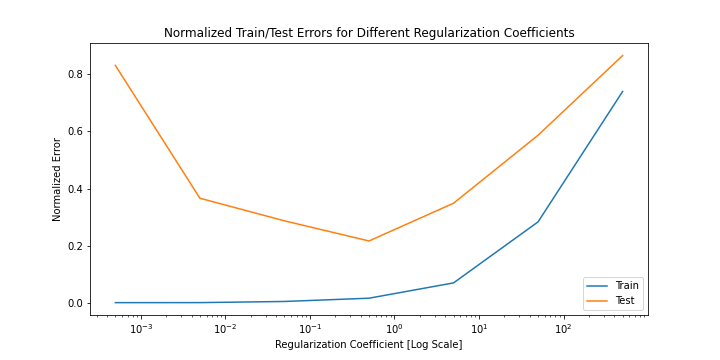
\includegraphics[scale=0.5]{figures/train_test_error_l2_reg.png}
      \caption{Train and Test Error as a function of different L2 Regularizers}
      \label{fig:train_test_error_l2}
    \end{figure}

    As we can see from the figure above, larger values of the $\lambda$ lead to an increase in the training error. Initially, they also lead to a \textit{decrease} in the test error, implying that the model is more adapt at generalizing. The sweet spot appears to be at a value of 0.5, where the test error is minimized. Larger values of the regulizer lead to an increase in both test and training errors, with a value of $500$ leading to a significant test and train error.

    In comparison to (a), we note that for intermediate values of $\lambda$, we achieve a significantly lower test error (~0.3), despite a slightly higher train error.

  \item
    The code we use builds up on the codes from Part 1 and Part 2. The only modifications are:
    \begin{verbatim}
def problem2c():
    for step_size in [0.00005,0.0005,0.005]:
        def sgd_solver(X, y, X_test, y_test):
            _, ahat = sgd(X, y, step_size=step_size, n_iters=int(1e6),
                          include_cost=False, include_detail=False)
            return ahat
        train, test, train_true, test_true = avg_train_test_error(n_trials=10, solver=sgd_solver)
        print("[step_size={}] Train Error: {:.4f}. Test Error: {:.4f}".format(step_size, train, test))
        print("[step_size={}] Train True Error: {:.4f}. Test True Error: {:.4f}".format(step_size, train_true, test_true))
      \end{verbatim}

      [step\_size=5e-05] Train Error: 0.0139. Test Error: 0.2618
      
      [step\_size=0.0005] Train Error: 0.0071. Test Error: 0.2662
      
      [step\_size=0.005] Train Error: 0.0038. Test Error: 0.4164


      As we can see from the results above, the all SGD solutions compare favorably to the optimal solution found with L2 regularization. They all achieve extremely low train errors (similar to optimal solution) and much better normalized test errors. In fact, for step sizes of 0.0005 and 0.00005, the test error of 0.22 is close or possibly even slightly lower than the optimal solution with L2 regularization factor of 0.5. This is because SGD serves as a regulizer, which means we no longer need an explicit L2 regularization factor. The randomness inhererint in SGD means that the model is far less likely to be caught in a local minimum, and it also serves to make sure the weights do not grow extremely large (since the loss signal is somewhat random).

    \item
      The code builds on top of the code from the previous parts. We have:
    \begin{verbatim}
def problem2d():
    for label, step_size in [("small", 0.00005), ("large", 0.005)]:
        normed_train_errors = []
        normed_test_errors = []
        a_norms = []
        n_iters=int(1e6)
        called = False
        def sgd_solver(X, y, X_test, y_test):
            nonlocal normed_train_errors, normed_test_errors, a_norms, called
            assert not called
            _, a_hat, normed_train_errors, normed_test_errors, a_norms = sgd(
                X, y, step_size=step_size, n_iters=n_iters, include_cost=False, include_detail=True,
                X_test=X_test, y_test=y_test)
            called = True
            return a_hat
        train, test, train_true, test_true = avg_train_test_error(n_trials=1, solver=sgd_solver)
        
        # Generate the three plots.
        # Train
        x_ticks = range(0, n_iters + 1, 100)
        plt.title("[step_size=%s] Normalized Training Error over SGD Train" % step_size)
        plt.xlabel("Iteration")
        plt.ylabel("Normalized Training Error")
        plt.plot(x_ticks, normed_train_errors, label="model")
        plt.plot(x_ticks, len(x_ticks) * [train_true], label="ground truth")
        plt.legend()
        plt.savefig("figures/training_error_for_iter_%s.png" % label, format="png")
        plt.close()
        
        # Test
        plt.title("[step_size=%s] Normalized Test Error over SGD Train" % step_size)
        plt.xlabel("Iteration")
        plt.ylabel("Normalized Test Error")
        plt.plot(x_ticks, normed_test_errors, label="model")
        plt.plot(x_ticks, len(x_ticks) * [test_true], label="ground truth")
        plt.legend()
        plt.savefig("figures/test_error_for_iter_%s.png" % label, format="png")
        plt.close()
        
        # Norm.
        plt.title("[step_size=%s] Solution Norm over SGD Train" % step_size)
        plt.xlabel("Iteration")
        plt.ylabel("Norm of Parameters")
        plt.plot(x_ticks, a_norms)
        plt.savefig("figures/solution_norms_for_iter_%s.png" % label, format="png")
        plt.close()

problem2d()
    \end{verbatim}

    We present the generated plots. For a small and converging step size of 0.00005, see Figure \ref{fig:sgd_iter_small}. For the larger and non-converging step size of 0.005, see Figure \ref{fig:sgd_iter_large}.

    \begin{figure}[!ht]
      \centering
      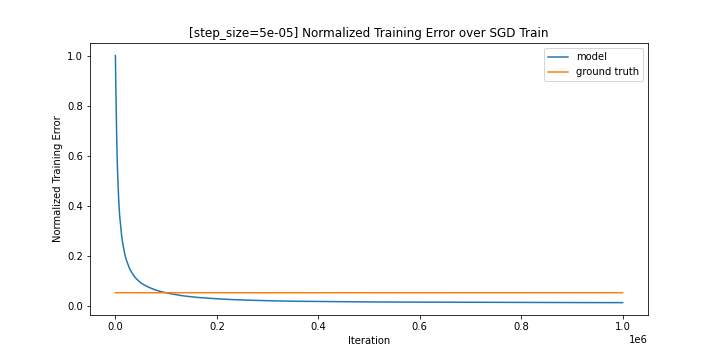
\includegraphics[scale=0.5]{figures/training_error_for_iter_small.png}
      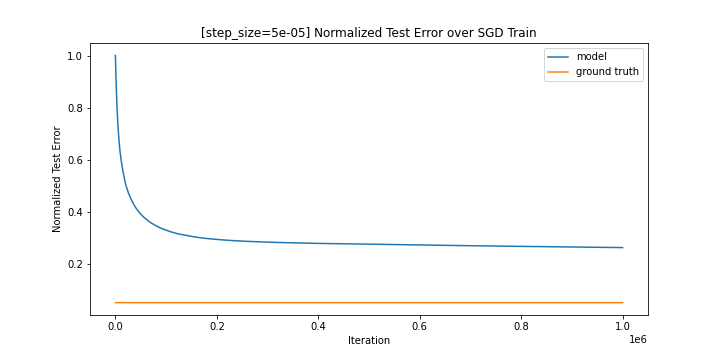
\includegraphics[scale=0.5]{figures/test_error_for_iter_small.png}
      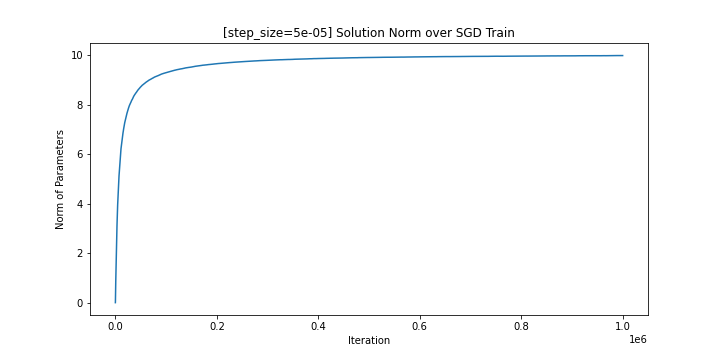
\includegraphics[scale=0.5]{figures/solution_norms_for_iter_small.png}
      \caption{Normalized Training Error, Normalized Test Error and model parameter norms over time as SGD training executes. We use a step size of 0.00005 for these plots.}
      \label{fig:sgd_iter_small}
    \end{figure}

    \begin{figure}[!ht]
      \centering
      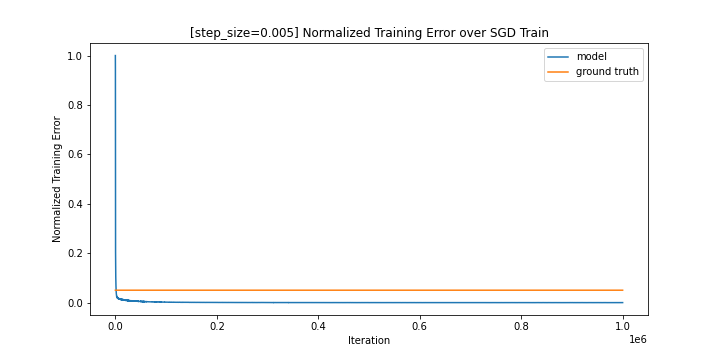
\includegraphics[scale=0.5]{figures/training_error_for_iter_large.png}
      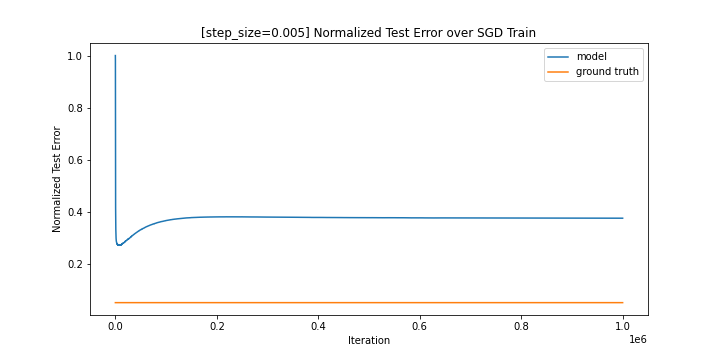
\includegraphics[scale=0.5]{figures/test_error_for_iter_large.png}
      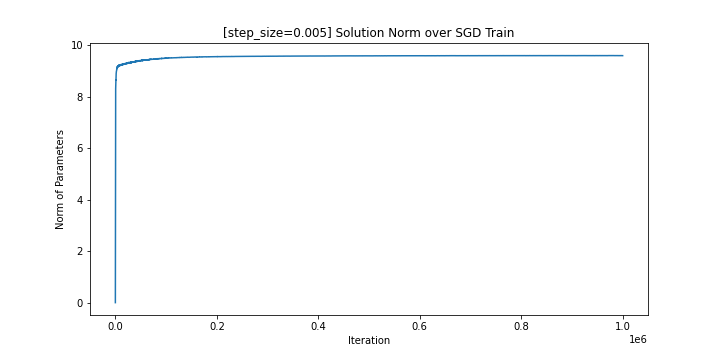
\includegraphics[scale=0.5]{figures/solution_norms_for_iter_large.png}
      \caption{Normalized Training Error, Normalized Test Error and model parameter norms over time as SGD training executes. We use a step size of 0.005 for these plots.}
      \label{fig:sgd_iter_large}
    \end{figure}

    From the plots above, we can see that the step size for SGD is critical to achiving good generilizeability. We can see from Figure \ref{fig:sgd_iter_large}, that too large a step size such as 0.005 initially reads to a rapid decrease in error. However, the model quickly begins overfitting to the training data, with the the relative test error increasing after about 20,000 or so iterations of SGD. Further interations simply lead to further overfitting. We also observe that the magnitude of the weights steadily increases.

    This in contrats to a more modest step size such as 0.00005 (see Figure \ref{fig:sgd_iter_small}). In this situation, the test error continue to decrease as we train. However, it does take much longer to achieve the same error as would have been achieved with the higher learning rate, but the learning is more stable. We also observe that the magnitude of the weights remains smaller than in the case where we overfit. 

    It is clear that the smaller $L_2$ norm appears to generalize better. However, our intuition that the model begins to overfit when the training error becomes too small does not really seem to match. In the case where our step size os $0.00005$, both the training and test errors continue to decrease (see Figure \ref{fig:sgd_iter_small}).

    \item
      The code used is presented below. Note that this builds on the code from previous parts.
      \begin{verbatim}
def initialize_random_sphere(d: int, r: int):
    """Random point in R^d chosen from r-sphere."""
    random = np.random.normal(size=(d,1))
    unit = random / np.linalg.norm(random)
    return r * unit

def problem2e():
    train_errors, test_errors = [], []
    rs = [0,0.1,0.5,1,10,20,30]
    for r in rs:
        def sgd_solver(X, y, X_test, y_test):
            _, ahat = sgd(X, y, step_size=0.00005, n_iters=int(1e6),
                          include_cost=False, include_detail=False,
                          initializer=lambda d: initialize_random_sphere(d, r))
            return ahat
        train, test, _, _ = avg_train_test_error(n_trials=10, solver=sgd_solver)
        print("[r={}] Train Error: {:.4f}. Test Error: {:.4f}".format(r, train, test))
        train_errors.append(train)
        test_errors.append(test)
    
    plt.title("Normalized Errors for Spherical Initialization")
    plt.xlabel("Sphere Radius [log]")
    plt.xscale('log')
    plt.ylabel("Normalized Error")
    plt.plot(rs, train_errors, label="train")
    plt.plot(rs, test_errors, label="test")
    plt.legend()
    plt.savefig("figures/spherical_initialization_log_x.png", format="png")
    plt.close()

problem2e()
      \end{verbatim}

      See Figure \ref{fig:spherical} for the plot.

      \begin{figure}
        \centering
        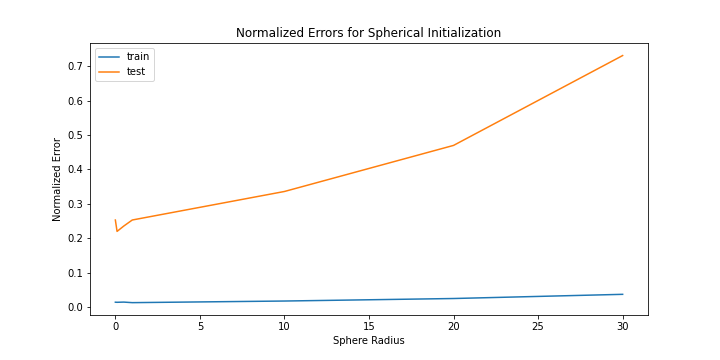
\includegraphics[scale=0.4]{figures/spherical_initialization.png}
        \caption{Train and Test Errors as a function of initialization values}.
        \label{fig:spherical}
      \end{figure}

    From the figure, we can see that as we increase the radius of our sphere, the test error increases significantly. The training error does not increase by much, however. In relation to (b), we suspect that this indicates a sort of regularization aspect caused by the initialization of the SGD near the origin of our space. Since we initialize with small weights, we are biased towards weights of smaller size while we do the search. On the other hand, if we initialize with larger weights, we're more likely to overfit the training data.
\end{enumerate}


\newpage
\section*{Part 3}
\begin{enumerate}[label=(\alph*)]
  \item
    We tried a deep learning approach. It didn't work. Code presented below:
    \begin{verbatim}
def initialize_parameters_deep(layer_dims):
    """
    Arguments:
    layer_dims -- python array (list) containing the dimensions of each layer in our network
    
    Returns:
    parameters -- python dictionary containing your parameters "W1", "b1", ..., "WL", "bL":
                    Wl -- weight matrix of shape (layer_dims[l], layer_dims[l-1])
                    bl -- bias vector of shape (layer_dims[l], 1)
    """
    parameters = {}
    L = len(layer_dims)

    for l in range(1, L):
        parameters['W' + str(l)] = np.random.randn(layer_dims[l], layer_dims[l-1]) * 0.01
        parameters['b' + str(l)] = np.zeros((layer_dims[l], 1))
        
        assert(parameters['W' + str(l)].shape == (layer_dims[l], layer_dims[l-1]))
        assert(parameters['b' + str(l)].shape == (layer_dims[l], 1))

        
    return parameters

def L_model_forward(X, Y, parameters):
    """
    Implement forward propagation for the [LINEAR->RELU]*(L-1)->LINEAR computation
    
    Arguments:
    X -- data, numpy array of shape (input size, number of examples)
    Y -- labels, numpy array of shape (1, number_of_examples)
    parameters -- output of initialize_parameters_deep()
    
    Returns:
    loss - the loss value after the forward pass.
    AL - final layer activations.
    caches -- list of caches containing:
                every cache of linear_activation_forward() (there are L-1 of them, indexed from 0 to L-1)
    """

    caches = []
    A = X
    L = len(parameters) // 2                  
    for l in range(1, L + 1):
        A_prev = A 
        W, b = parameters['W' + str(l)], parameters['b' + str(l)]
        Z = np.dot(W, A) + b
        # Last layer is just linear w/o ReLU
        A = np.maximum(Z, 0) if l < L else Z
        # There are used in the backawards pass for derivative calculations.
        caches.append((Z, A_prev, W))
    
    assert(A.shape == (1,X.shape[1]))
    
    cost = np.mean((A - Y)**2)
            
    return cost, A, caches

def L_model_backward(AL, Y, caches):
    """
    Implement the backward propagation for the [LINEAR->RELU] * L
    
    Arguments:
    AL -- vector, output of the forward propagation (L_model_forward())
    Y -- true "label" vector (containing 0 if non-cat, 1 if cat)
    caches -- list of caches containing:
                every cache of linear_activation_forward()
    
    Returns:
    grads -- A dictionary with the gradients
             grads["dA" + str(l)] = ... 
             grads["dW" + str(l)] = ...
             grads["db" + str(l)] = ... 
    """
    grads = {}
    L = len(caches)
    m = AL.shape[1]
    Y = Y.reshape(AL.shape)
    
    # Initializing the backpropagation
    grads["dA" + str(L)] = 2 * (AL - Y)
    
    # Loop from l=L-1 to l=0
    for l in reversed(range(L)):
        Z, A, W = caches[l]
        dZ = grads["dA" + str(l + 1)]
        if l < L - 1:
            # Final layer is just linear, so all units go through.
            dZ[Z < 0] = 0
        grads["dW" + str(l+1)] = np.dot(dZ, A.T)
        grads["db" + str(l+1)] = np.sum(dZ, axis=1, keepdims=True)
        grads["dA" + str(l)] = np.dot(W.T, dZ)

    return grads

def deep_net_solver(X_train, y_train, layer_dims, batch_size, n_epochs, lr=0.001, l2_coeff=0.0):
    """Implement mini-batch SGD.
    
    Args:
        X_train: (f, n) matrix.
        y_train: (1, n) matrix.
        layers_dims: The size of each layer in the networks. 
        batch_size: batches of elements to take for SGD.
        n_epochs: Number of iterations over the dataset to execute.
        lr: learning rate
        l2_coeff: l2_coefficient for regularization.
    """
    f, n = X_train.shape
    batches_per_epoch = n // batch_size + (1 if n % batch_size != 0 else 0)
    parameters = initialize_parameters_deep(layer_dims)
    costs = []
    t_costs = []
    for epoch in range(n_epochs):
        idxs = np.arange(n)
        np.random.shuffle(idxs)
        X_shuffled = X_train[:, idxs]
        y_shuffled = y_train[:, idxs]
        for i in range(batches_per_epoch):
            X = X_shuffled[:, batch_size * i: batch_size * (i+1) if i + 1 < batches_per_epoch else None]
            y = y_shuffled[:, batch_size * i: batch_size * (i+1) if i + 1 < batches_per_epoch else None]
            _, AL, caches = L_model_forward(X, y, parameters)
            grads = L_model_backward(AL, y, caches)
            
            # Update parameters.
            for name, param in parameters.items():
                parameters[name] = param - lr * (grads["d" + name] + 2 * l2_coeff * param)
    
        # Loss on train set.
        _, A, _ = L_model_forward(X_train, y_train, parameters)
        cost = np.linalg.norm(A - y_train) / np.linalg.norm(y_train)
        costs.append(cost)
        print("Relative Train Error after {} epochs: {:.4f}.".format(epoch + 1, cost))
    return costs, parameters

X_train, y_train, X_test, y_test, a_true = generate_data_3()

deep_net_solver(X_train.T, y_train.T, [200, 100, 50, 25, 1], batch_size=8, n_epochs=100, lr=0.0005, l2_coeff=0.5)
    \end{verbatim}

    The deep learning approach achieved a low train error (< 0.06), but we were not able to have this approach generalize. The relative test error stood at 13.8082.
    \begin{verbatim}
def problem3a():
    normed_train_errors = []
    normed_test_errors = []
    a_norms = []
    def local_solver(X, y, X_test, y_test):
        nonlocal normed_train_errors, normed_test_errors, a_norms
        costs, a_hat, normed_train_errors, normed_test_errors, a_norms = sgd(
            X, y, step_size=0.0005, n_iters=int(2e4), include_cost=False, include_detail=True,
            X_test=X_test, y_test=y_test)
        return a_hat
    train, test, _, _ = avg_train_test_error(n_trials=200, solver=local_solver, data=generate_data_3)
    return normed_train_errors, normed_test_errors, train, test

trains, tests, train, test = problem3a()

plt.plot(range(len(trains)), trains, label="train")
plt.plot(range(len(tests)), tests, label="test")
    \end{verbatim}

    Instead, our best-performing approach consisted of simply using SGD with an aptly chosen step size of 0.0005 and trained for 20,000 iterations. This gave us a final average (over 200 trials) relative test error of:
    \[
      0.7070012887366063
    \]
    and corresponding average relative train error of:
    \[
      0.0008997399081278824
    \]

    We reasoned that SGD served as a sufficiently strong regularizer, based on the results from the previous parts. As such, we opted not to use any explicit regularization in the model, instead directly optimizing for the value we were interested in. We focused exclusively on finding good step values for SGD, discovering the optimal one to be 0.0005 which resulted in a relatively low test rate. We also verified that our model was not overfitting, by making plots (see appendix).

  \item
    Following the approach from 3a, we decided to similar stick to just using SGD alone (rather than explicit regularization).

    We tried a few things, but most did not seem to help. In particular, we tried changing the final answer by randomly rounding the values to enforce sparsity (values < 0.9 would be 0, values > 0.9 would be 1.0). This did not help however. 

    In the end, we ended with a test error of:
    \[
      0.7070012887366063
    \]

\end{enumerate}


\newpage
\section*{Appendix}
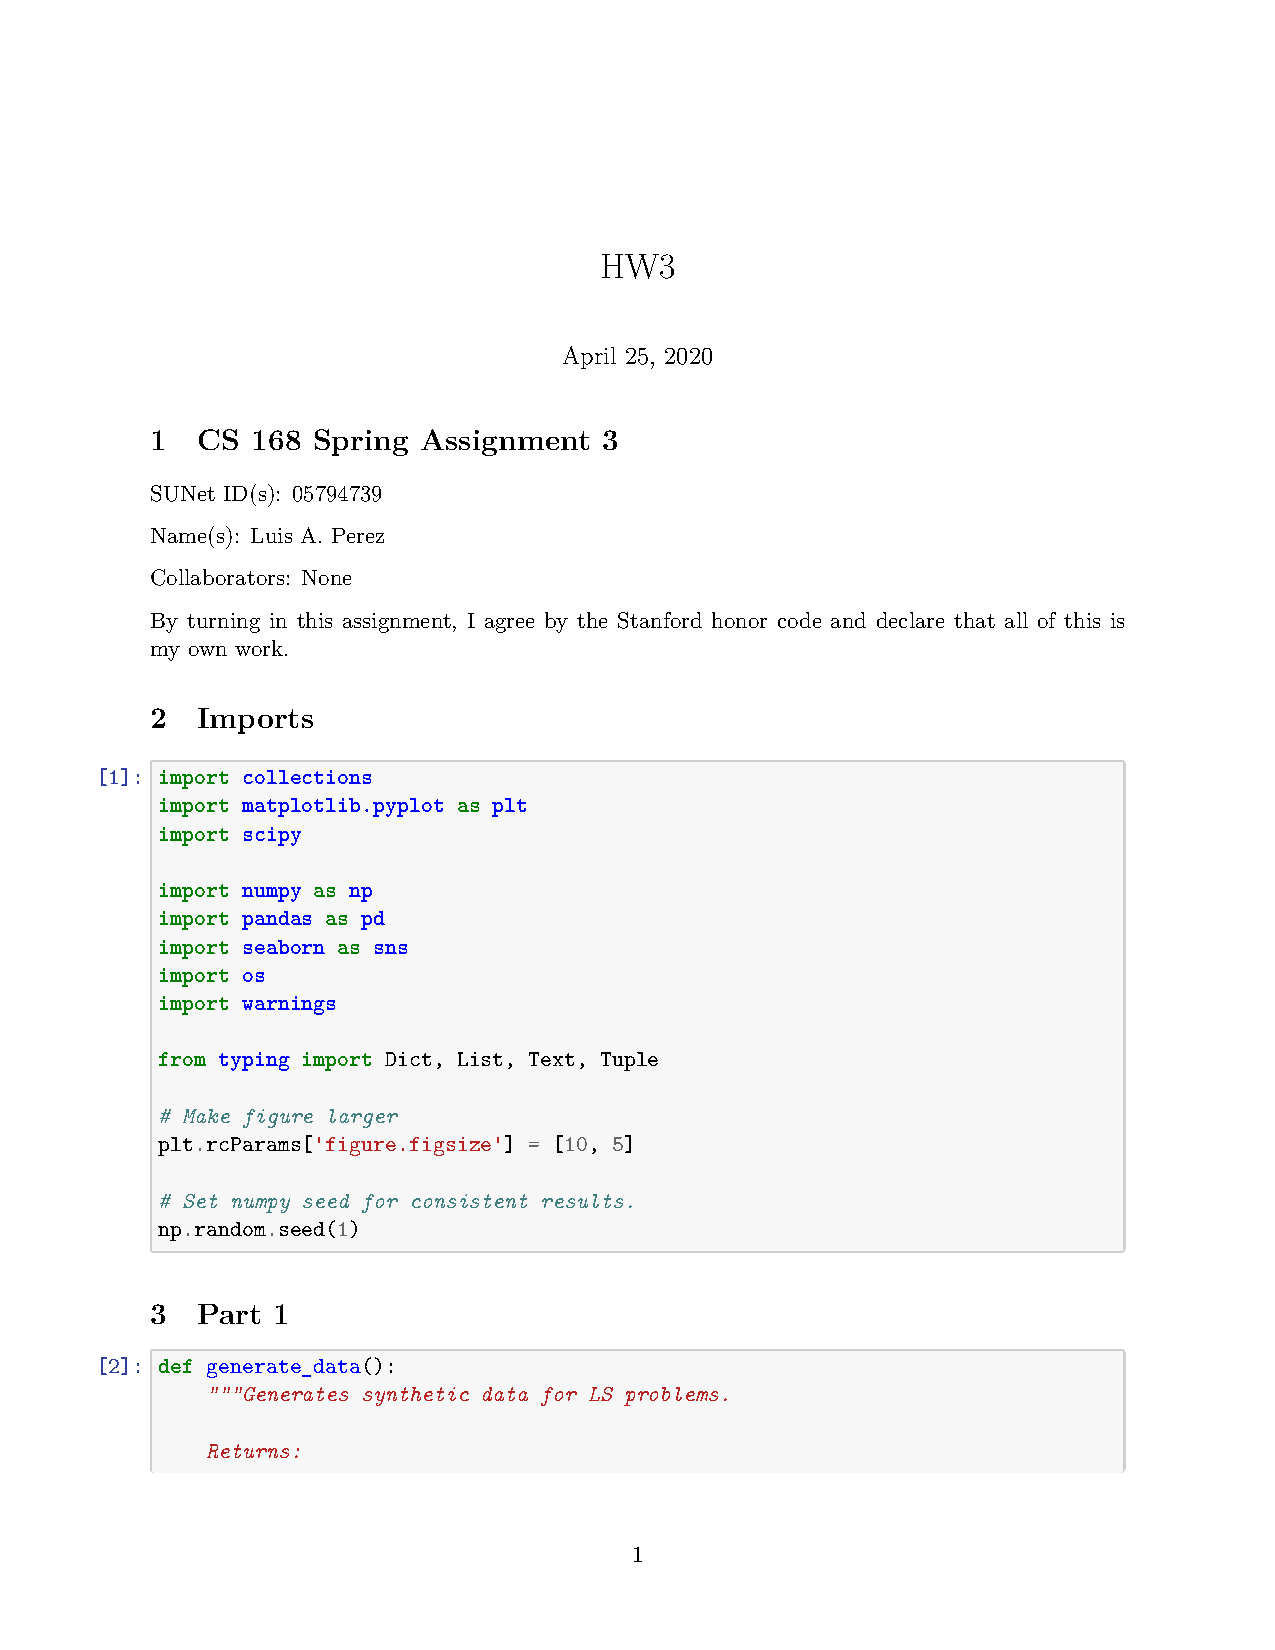
\includepdf[pages=-]{HW3}

\end{document}
